In this section we will explain our how our model works and the approached we have used. First we will explain the interactions between the shark and fish before we go in to a more detailed description of how the fish and shark models work.

The fish model used is a combination of previously used models with our own modifications to it. We have created a model of the shark based on multi layer feed forward artificial neural network, trained using a evolutionary  algorithm.

Since we are only interested in modeling the shark when it is hunting we choose to limit our model to only include the phase where the shark has visual contact with the fish shoal. This gives the advantage that we can stop the evaluation in training of sharks that go to far away from the fish. It also let us consider an infinite large sea. The fish are free to move around in the sea without any boundary or periodic boundary. This gives a large performance gain in the training of the neural network.

The movement of the fish and shark is not constrained by any structure or grid. It can however only have discrete coordinates. It is also limited by the model of the animal itself as will be explained below.

The shark and fish shoal positions are updated asynchronously, but the fish in the shoal is updated synchronously. If the shark moves to the position of a fish, the fish is considered eaten by the shark and is as a result removed from the shoal.

To compare if the the shark we accure from the evolutionare based training is succsesfull we compare it to a shark that uses a more straight forward approached.

Now we will proceed to the more detailed descriptions of the fish and shark models.

\subsection{The fish shoal}

\begin{figure}
\centering
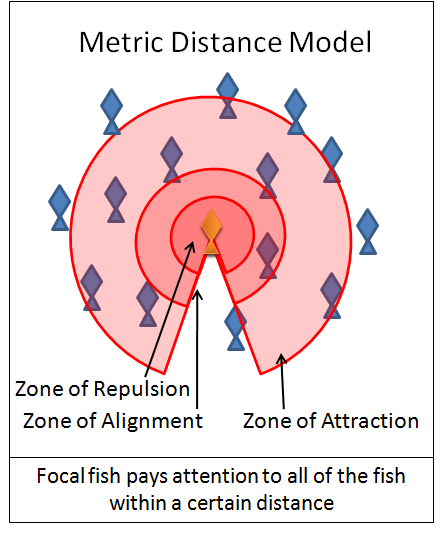
\includegraphics[width=0.45\textwidth]{figs/swarmfig.png}
\caption{\label{fig:swarm} Fish shoal model.}
\end{figure}

The swarming model used is based on the two models found in the references \cite{javafish} and \cite{matlabfish}. It follows the same rules as the basic swarming model, namely repulsion, alignment and attraction. Each of these rules applies at a certain distance range from the fish which can be seen in figure \ref{fig:swarm}. If another fish enters the zone of repulsion they will tend to repel each other and not surprisingly if they are within the attraction distance, they will tend to move towards each other. In the zone of alignment they tend to align themselves so that they will move in the same direction as the other fish in that zone. Behind the fish there is also a dead zone where no interaction occur (most animals can not see things behind themselves). To further improve the behavior of the swarm, there is also an addition to the algorithm called distance priority \cite{matlabfish}. It makes the fish tend to align itself to the average direction of a set number of its closest neighbors, regardless of which zone they are in.\\
\\
The fish in the shoal move at a constant drift speed but can accelerate to a max speed to avoid the shark. The way the fish in this model avoids the shark is quite simple. A scare distance is set for the fish and should the predator be within this distance, the fish will completely ignore the swarming rules and update the velocity according to
\begin{equation}
\vec{v}_f \rightarrow \vec{v}_f - (\vec{x}_s - \vec{x}_f)a
\end{equation}
where $\vec{v}_f$ is the velocity of the fish, $\vec{x}_s$ the position of the shark, $\vec{x}_f$ the position of the fish and $a$ is a constant called acceleration rate, which decides how fast the fish will be able to reach its max speed (note that the time step is excluded since it will always be set to 1). In other words the fish will just move in opposite direction of where the shark is relative to itself starting at its drift speed and accelerating to its max speed. Having the avoidance rule this way makes for a problem however since this could force a fish to move outside of the attraction zone of the fish furthest out in the shoal. To solve this it is added that should a fish get too far away from the center of the shoal (average position of all fish), it will move strictly towards this point if not too close to the shark.

\subsection{The shark}

The model we have created is inspired by nature but not is not an exact description of how sharks behave.

The shark has many senses it can use to detect prey, even on large distances using sight, smell, hearing, electro reception and by detecting vibrations in water, more about this in \cite{shark_vision} and \cite{shark_electric}. Since we have limited ourself to the actual fish catching phase of the hunting we are not interested in the long distance senses.  It is unknown exactly how the all the sharks senses work and it is therefore  difficult to model them, we have chosen an approach that symbolize a combination of the senses in a single sense. The sense model was in our case also limited by the kind of input that were usable with the neural network. The model allows the shark to perceive a fish shoal in front and back of the shark separately as well as the closest fish in the area where the shark is able to catch the fish.

Even though the shark is a very agile predator it can not turn in full speed on the spot, we have therefore constrained the sharks turning angle so that it can only turn $\pi/4$ in each time step. This means that a shark moving at greater speeds will need a larger area for turning.

The parameters of the shark are:
\begin{itemize}
\item observe distance
\item max step size
\item energy reserve
\end{itemize}

\subsubsection{The brain -- artificial neural network}
\begin{figure}
\centering
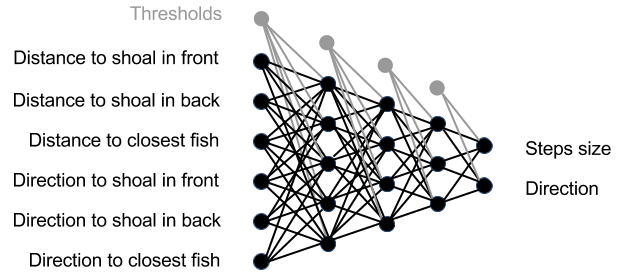
\includegraphics[width=.7\textwidth]{figs/ann_structure.png}
\caption{\label{fig:ann}}
\end{figure}

Our shark behavior is controlled by an Artificial neural network, ANN. The inputs to the network as can be seen in Figure \ref{fig:ann} is the center of the fish shoal in front and back as well as the position of the closest fish within the sharks attack area (the sector in front of the shark with angle $\frac{\pi}{2}$ up to the sharks maximum movement distance). The positions are given to the network in polar coordinates relative to the sharks position and direction, normalized between zero and unity. The distances are 0 when the position is at the furthers position and 1 at the same position as the shark. The angles are 0 when on the right edge of the sector and 1 when on the left edge of the sector. When in front of the shark the angle is 0.5.

The output from the network is also given in normalized polar coordinates relative to the shark where steps size 1 means maximum step size. The direction is normalized in the same way as the input.

The network consist of the 6 input neurons explained above, 3 hidden layers with one neuron less than the previous layers and 2 output neurons also explained above. In addition to this, each layer (except for the output layer) has an extra neuron with input constant 1. This extra neurons acts as the threshold.

The network was trained using an evolutionary genetically algorithm with real number encoding, crossover, mutation and elite inserts starting from a random population.

In each generation of the training, each individual is given a fitness value based on an evaluation where the sharks is hunting fish as described earlier.

Since the shark is a predator and as such its success in hunting can be measured by the amount of energy spent on the hunt in regards to how much energy it could consume from the prey caught. We used the fitness calculated as follow for each individual:

\begin{equation}
  F = S+D\label{eq:fitness}
\end{equation}
where $S$ is the number of fish caught by the shark and $D$ is the average distance to the center of the closest fish shoal normalized between zero and unity. The distance is part of the fitness calculation to remove the discreteness. This helps to differentiate between individuals that caught the same amount of fish, especially in the beginning of the training where no fish are caught.

The fitness value itself does not contain any information about how much energy it spent catching its prey, instead this is handled by the stop condition that the shark only has a certain amount of energy to spend before the evaluation is stopped. The evaluation can also be stopped if the shark loses contact with the fish. The energy is calculated as distanced moved. Therefore a shark that turn in a greater speed consumes more energy than a shark that turns in slower speed, due to that the faster moving shark needs a larger area to turn on.

\subsection{Shark for comparison}
The fitness value of the shark is great to compare different shark, but how do we tell if the shark with the best fitness value is good, decent or bad. We can look at the visual representation of the shark hunting and judge from its behavior, to conclude if it is good or bad. Another approached that is a bit less heuristic is to compare it with a hard coded algorithm instead of the ANN. The inputs and outputs to this algorithm we came up with is the same as to the ANN. The algorithm can be described:
\begin{enumerate}
\item If the distance to the closest fish is not zero (fish in attack area):\\
    \hspace*{5pt}Eat that fish.
\item Else if fish shoal in front of shark and within move angle: \\
    \hspace*{5pt}Let output be the polar coordinates to the fish shoal in front.
\item Else if fish shoal in front of shark and not within move angle: \\
    \hspace*{5pt}Move with maximum angle toward the fish shoal with 20\% of max speed.
\item Else if fish shoal in back:\\
    \hspace*{5pt}Move with maximum angle to the side that is closes to the fish shoal with 20\% of max speed.
\end{enumerate}

